%%%%%%%%%%%%%%%%%%% vorlage.tex %%%%%%%%%%%%%%%%%%%%%%%%%%%%%
%
% LaTeX-Vorlage zur Erstellung von Projekt-Dokumentationen
% im Fachbereich Informatik der Hochschule Trier
%
% Basis: Vorlage svmono des Springer Verlags
%
%%%%%%%%%%%%%%%%%%%%%%%%%%%%%%%%%%%%%%%%%%%%%%%%%%%%%%%%%%%%%

\documentclass[envcountsame,envcountchap, deutsch]{i-studis}

\usepackage{makeidx}         	% Index
\usepackage{multicol}        	% Zweispaltiger Index
%\usepackage[bottom]{footmisc}	% Erzeugung von Fu�noten

%%-----------------------------------------------------
%\newif\ifpdf
%\ifx\pdfoutput\undefined
%\pdffalse
%\else
%\pdfoutput=1
%\pdftrue
%\fi
%%--------------------------------------------------------
%\ifpdf
\usepackage[pdftex]{graphicx}
\usepackage{epstopdf}
\usepackage[pdftex,plainpages=false]{hyperref}
%\else
%\usepackage{graphicx}
%\usepackage[plainpages=false]{hyperref}
%\fi

%%-----------------------------------------------------
\usepackage{color}				% Farbverwaltung
%\usepackage{ngerman} 			% Neue deutsche Rechtsschreibung
\usepackage[english, ngerman]{babel}
\usepackage[latin1]{inputenc} 	% Erm�glicht Umlaute-Darstellung
%\usepackage[utf8]{inputenc}  	% Erm�glicht Umlaute-Darstellung unter Linux (je nach verwendetem Format)

%-----------------------------------------------------
\usepackage{listings} 			% Code-Darstellung
\lstset
{
	basicstyle=\scriptsize, 	% print whole listing small
	keywordstyle=\color{blue}\bfseries,
								% underlined bold black keywords
	identifierstyle=, 			% nothing happens
	commentstyle=\color{red}, 	% white comments
	stringstyle=\ttfamily, 		% typewriter type for strings
	showstringspaces=false, 	% no special string spaces
	framexleftmargin=7mm, 
	tabsize=3,
	showtabs=false,
	frame=single, 
	rulesepcolor=\color{blue},
	numbers=left,
	linewidth=146mm,
	xleftmargin=8mm
}
\usepackage{textcomp} 			% Celsius-Darstellung
\usepackage{amssymb,amsfonts,amstext,amsmath}	% Mathematische Symbole
\usepackage[german, ruled, vlined]{algorithm2e}
\usepackage[a4paper]{geometry} % Andere Formatierung
\usepackage{bibgerm}
\usepackage{array}
\hyphenation{Ele-men-tar-ob-jek-te  ab-ge-tas-tet Aus-wer-tung House-holder-Matrix Le-ast-Squa-res-Al-go-ri-th-men} 		% Weitere Silbentrennung bei Bedarf angeben
\setlength{\textheight}{1.1\textheight}
\pagestyle{myheadings} 			% Erzeugt selbstdefinierte Kopfzeile
\makeindex 						% Index-Erstellung


%--------------------------------------------------------------------------
\begin{document}
%------------------------- Titelblatt -------------------------------------
\title{Titel der Arbeit auf Deutsch}
\subtitle{English Title}
%---- Die Art der Dokumentation kann hier ausgew�hlt werden---------------
%\project{Bachelor-Projektarbeit}
\project{Bachelor-Abschlussarbeit}
%\project{Master-Projektstudium}
%\project{Master-Abschlussarbeit}
%\project{Seminar zur Vorlesung ...}
%\project{Hausarbeit zur Vorlesung ...}
%--------------------------------------------------------------------------
\supervisor{Titel Vorname Name} 		% Betreuer der Arbeit
\author{Autor} 							% Autor der Arbeit
\address{Ort,} 							% Im Zusammenhang mit dem Datum wird hinter dem Ort ein Komma angegeben
\submitdate{Abgabedatum} 				% Abgabedatum
%\begingroup
%  \renewcommand{\thepage}{title}
%  \mytitlepage
%  \newpage
%\endgroup
\begingroup
  \renewcommand{\thepage}{Titel}
  \mytitlepage
  \newpage
\endgroup
%--------------------------------------------------------------------------
\frontmatter 
%--------------------------------------------------------------------------
\preface

Ein Vorwort ist nicht unbedingt n�tig. Falls Sie ein Vorwort schreiben, so ist dies der Platz, um z.B. die Firma vorzustellen, in der diese Arbeit entstanden ist, oder einigen Leuten zu danken, die in irgendeiner Form positiv zur Entstehung dieser Arbeit beigetragen haben. Auf keinen Fall sollten Sie im Vorwort die Aufgabenstellung n�her erl�utern oder vertieft auf technische Sachverhalte eingehen.				% Vorwort (optional)
\kurzfassung

%% deutsch
\paragraph*{}
%In der Kurzfassung soll in kurzer und pr�gnanter Weise der wesentliche Inhalt der Arbeit beschrieben werden. Dazu z�hlen vor allem eine kurze Aufgabenbeschreibung, der L�sungsansatz sowie die wesentlichen Ergebnisse der Arbeit. Ein h�ufiger Fehler f�r die Kurzfassung ist, dass lediglich die Aufgabenbeschreibung (d.h. das Problem) in Kurzform vorgelegt wird. Die Kurzfassung soll aber die gesamte Arbeit widerspiegeln. Deshalb sind vor allem die erzielten Ergebnisse darzustellen. Die Kurzfassung soll etwa eine halbe bis ganze DIN-A4-Seite umfassen.

%Hinweis: Schreiben Sie die Kurzfassung am Ende der Arbeit, denn eventuell ist Ihnen beim Schreiben erst vollends klar geworden, was das Wesentliche der Arbeit ist bzw. welche Schwerpunkte Sie bei der Arbeit gesetzt haben. Andernfalls laufen Sie Gefahr, dass die Kurzfassung nicht zum Rest der Arbeit passt.



Diese Arbeit befasst sich mit der Konzeption und Realisierung eines Information-Retrieval-Systems, welches ein Archiv mit semistrukturierten Dokumenten, die sowohl Freitext als auch Metadaten enthalten, effizient nach vom Nutzer festgelegten und logisch verkn�pfbaren Kriterien durchsucht. Ziel der Implementierung ist es, dem Nutzer nach Abschluss des Suchvorgangs zu seinem Informationsbed�rfnis passende Dokumente zur�ckzuliefern und diese auf eine �bersichtliche Weise zu pr�sentieren. \\
Zun�chst wird die Problemstellung im Detail erl�utert, damit der Leser eine genaue Vorstellung �ber die Anforderungen, welche die Implementierung erf�llen soll, bekommt. Anschlie�end wird Information Retrieval im Allgemeinen vorgestellt, um einen �berblick �ber die Thematik zu geben. 
Es folgt eine Vorstellung der beiden klassischen Information Retrieval Modelle boolesches Retrieval und Vektorraummodell inklusive Erl�uterung der Funktionsweisen. Anschlie�end wird beschrieben, wie sich solche Modelle in Hinsicht auf deren Qualit�t bewerten und vergleichen lassen.\\
Nach dem Vermitteln der notwendigen theoretischen Kenntnisse beschreibt der Implementierungsteil, auf welche Weise und in welchen Bereichen die beiden Verfahren f�r die Implementierung zum Einsatz kamen und inwieweit eine Modifizierung zur Anpassung auf die vorliegende Problemstellung erfolgte. 
Neben der internen Funktionsweise wird auch die Benutzung der Oberfl�che erl�utert, um den Anwender mit der Bedienung des Systems vertraut zu machen.  \\
Es folgt eine Zusammenfassung der Arbeit mit abschlie�ender Bewertung der Ergebnisse sowie ein Ausblick auf zuk�nftige Verbesserungsm�glichkeiten.
\newpage
\paragraph*{}
This paper discusses the conception and realization of an information retrieval system that searches efficiently in semistructured data containing free text and metadata. The  search criteria for this system are determined by the user and can be freely connected with boolean operators. The aim of the implementation is to retrieve documents satysfying the user's information need and to present the results clearly.\\
First the problem is discussed in detail to give the reader a precise idea of the requirements which the implementation has to fit. Afterwards, information retrieval in general is presented to give an overview on the topic.
The chapter about information retrieval is followed by a presentation of two classical information retrieval model including their functionality called boolean retrieval and vectorspace model. Afterwards, it is discussed how the quality of such systems can be estimated and compared. \\
After having provided the necessary theory, the paper continues with the implementation part, which explains which models were used in which way and if they have been modified in any way to fit this problem. 
Aside from the intern functionality, the reader learns about how to operate with the system via the given user interface. \\
The paper concludes with a summary including a final result evaluation and a presentation of future prospects for system improvements.




 			% Kurzfassung Deutsch/English
\tableofcontents 						% Inhaltsverzeichnis
\listoffigures 							% Abbildungsverzeichnis (optional)
\listoftables 							% Tabellenverzeichnis (optional)
%--------------------------------------------------------------------------
\mainmatter                        		% Hauptteil (ab hier arab. Seitenzahlen)
%--------------------------------------------------------------------------
% Die Kapitel werden in separaten .tex-Dateien abgelegt und hier eingebunden.
\chapter{Einleitung und Problemstellung}

\section{Einleitung}

Wer kennt es nicht: Tagt�glich treffen neue E-Mails ein, sodass das Postfach sich immer weiter f�llt. \\
Schnell ist es passiert, dass die Menge an Nachrichten un�bersichtlich gro� wird, was zu einem ernsthaften Problem wird, sobald man etwas bestimmtes darin wiederfinden m�chte. \\
Die ben�tigte Mail war wichtig, weil sie eine bestimmte Kontaktadresse enthielt, aber wie war nochmal der Absender? L�ngst vergessen. Das genaue Datum? Leider ist nur noch der Monat bekannt. Wer jetzt manuell suchen muss, ist an dieser Stelle verloren. \\
Abhilfe schafft ein Information Retrieval System, mit dem man bestimmte Suchkriterien eingeben und beliebig miteinander kombinieren kann. \\
 So bekommt der Nutzer genau die Nachrichten pr�sentiert, die sein Informationsbed�rfnis am ehesten bedienen, und  braucht sich nicht erst durch hunderte von Mails durchzuarbeiten. In diesem Fall k�nnte die Person beispielsweise im Freitext nach dem Wort \glqq Kontaktadresse\grqq{} suchen und weitere Kriterien wie \glqq Datum = Juni \grqq{} hinzuf�gen. \\
Besonderheit ist das beliebige Verkn�pfen: Der Nutzer kann sich entscheiden, ob er nur Resultate akzeptiert, auf die Beides zutrifft, oder ob es bereits reicht, wenn eines der Kriterien erf�llt ist. Dies erlaubt eine sehr individuelle, auf den Benutzer zugeschnittene Suche. \\
Ein solches System ist nicht nur f�r das Alltagsbeispiel E-Mail-Ordner, d.h. Posteingang, Postausgang etc. wertvoll, sondern l�sst sich auch auf jede andere Art von Dokumentenarchiv, dessen Dokumente sowohl Freitext als auch Metadaten beinhalten, anwenden. 





\section{Problemstellung}

Ziel der Arbeit ist die Konzeption und Realisierung eines Systems zur Informationssuche (engl. Information Retrieval System) in einem Dokumentenarchiv, wobei die Dokumente von teilweise strukturierter Natur sind. \\
Dies bedeutet, dass sie sowohl gew�hnlichen Freitext als auch Metadaten enthalten. Der Nutzer soll spezifizieren k�nnen, in welchen Metadaten er suchen m�chte, zudem soll die Freitextsuche ausw�hlbar sein. Alle Suchanfragen sollen hierbei beliebig mit den booleschen Operatoren \textit{AND} (engl. und) sowie \textit{OR} (engl. oder) verkn�pfbar sein. \\
Hauptanwendungszweck des Systems sind E-Mail-Archive wie Posteingang und Postausgang, allerdings soll das System so flexibel sein, dass es auch auf andere teilweise strukturierte Dokumentenarchive anwendbar ist. 


\section{Teilprobleme}
Aus der Aufgabenstellung ergeben sich die im folgenden beschriebenen Teilprobleme.


\subsection{Dynamisches einlesen der Metadaten}
Die genauen Metadaten sind, da das System flexibel sein soll, vor dem Ausf�hren des Systems noch nicht bekannt. Demnach muss das IR-System die Namen der Metadaten beim Starten des Programms dynamisch einlesen und diese dem Nutzer auf der grafischen Oberfl�che anzeigen.

\subsection{Unterscheidung Metadaten und Freitext}
Damit das System die Metadaten dynamisch einlesen kann, m�ssen die folgenden Punkte erf�llt sein:
\begin{enumerate}
	\item Das System muss zwischen Metadaten und Freitext unterscheiden k�nnen.
	\item Metadaten setzen sich aus Name und Inhalt zusammen, weshalb beides erkannt und voneinander abgegrenzt werden muss. Im folgenden werden die Namen als \glqq Keywords \grqq{} bezeichnet.
	\item Der Inhalt kann unterschiedlichen Datentyps sein, z.B. String oder Liste, weshalb dieser bestimmt werden muss.
\end{enumerate}


\subsection{Metadatensuche}
Es muss erkannt werden, welche Metadaten der Nutzer ausgew�hlt hat und in genau diesen muss, unter Ber�cksichtigung des jeweiligen Datentyps der Inhalte, gesucht werden. \\
Im Gegensatz zur Freitextsuche muss zu jedem Dokument vor der Suche zun�chst gepr�ft werden, ob das entsprechende Schl�sselwort �berhaupt darin auftritt.

\subsection{Freitextsuche}
Bei der Freitextsuche ist die Wortzahl weitaus gr��er als bei der Metadatensuche. Daraus resultieren zwei Probleme:
\begin {enumerate}
\item Wie kann effizient in gro�en Wortmengen gesucht werden?
\item Wie kann die Suche bei begrenztem Speicher bew�ltigt werden?
\end{enumerate}

Zudem stellt sich die Frage nach einem geeigneten Verfahren, das bei l�ngeren Anfragen auch teilweise passende Ergebnisse liefert und messen kann, wie gut die erzielten Treffer zur Nutzeranfrage passen.


\subsection{Verkn�pfung mit UND/ODER}
Alle Anfragen sollen beliebig mit den logischen Operatoren \textit{AND}, \textit{OR} sowie \textit{NOT} verkn�pfbar sein. Dies beinhaltet die folgenden Problemstellungen:
\begin{enumerate}
\item Keywordsuche und Freitextsuche m�ssen miteinander verkn�pft werden.
\item Sind meherere Keywords ausgew�hlt, m�ssen die Teilergebnisse verkn�pft werden.
\item Stellt der Nutzer mehrere Anfragen, m�ssen die Ergebnisse der einzelnen Anfragen verkn�pft werden.
	\end{enumerate}






\subsection{Benutzeroberfl�che}
Der Nutzer ben�tigt eine verst�ndliche Benutzeroberfl�che, die es ihm erm�glicht, seine Suchanfragen beliebig zusammenzustellen. Hierzu muss die Oberfl�che folgende grundlegenden Funktionalit�ten aufweisen:
\begin{enumerate}
	\item Das Suchverzeichnis, d.h. das Dokumentenarchiv in welchem die Suche stattfindet, muss ausw�hlbar sein. 
	\item Alle im Archiv auftretenden Keywords sowie die Freitextsuche m�ssen ausw�hlbar sein.
	\item Logische Operatoren (AND,OR,NOT) zur Verkn�pfung m�ssen ausw�hlbar sein.
	\item Die Suchanfrage muss f�r den Nutzer verst�ndlich angezeigt werden.
	
	
\end{enumerate}

\chapter{Weitere Kapitel}

Die Gliederung h�ngt nat�rlich vom Thema und von der L�sungsstrategie ab. Als n�tzliche
Anhaltspunkte k�nnen die Entwicklungsstufen oder - schritte z.B. der Softwareentwicklung betrachtet werden. N�tzliche Gesichtspunkte erh�lt und erkennt man, wenn man sich
\begin{itemize}
  \item in die Rolle des Lesers oder
  \item in die Rolle des Entwicklers, der die Arbeit z.B. fortsetzen, erg�nzen oder pflegen soll,
\end{itemize}
versetzt. In der Regel wird vorausgesetzt, dass die Leser einen fachlichen Hintergrund haben - z.B. Informatik studiert haben. D.h. nur in besonderen, abgesprochenen F�llen schreibt man in popul�rer Sprache, so dass auch Nicht-Fachleute die Ausarbeitung prinzipiell lesen und verstehen k�nnen.

Die �u�ere Gestaltung der Ausarbeitung hinsichtlich Abschnittformate, Abbildungen, mathematische Formeln usw. wird in \hyperref[Stile]{Kapitel~\ref*{Stile}} kurz dargestellt.
\chapter{LaTeX-Bausteine}\label{Stile}

Der Text wird in bis zu drei Ebenen gegliedert:

\begin{enumerate}
  \item Kapitel ( \verb \chapter{Kapitel} ), \index{Kapitel}
  \item Unterkapitel  ( \verb \section{Abschnitt} ) und
  \item Unterunterkapitel  ( \verb \subsection{Unterabschnitte} ).
\end{enumerate}

\section{Abschnitt}\index{Abschnitt}
Text der Gliederungsebene 2.


\subsection{Unterabschnitt} \index{Unterabschnitt}
Text der Gliederungsebene 3.
Text Text Text Text Text Text Text Text Text Text Text Text Text Text Text
Beispiel f�r Quelltext\index{Quelltext} \\[2 ex]
\noindent
\begin{minipage}{1.0\textwidth} \small
\begin{lstlisting}
	Prozess 1:
	
	Acquire();
		a := 1;
	Release();
	...
	Acquire();
	if(b == 0)
	{					
		c := 3;
		d := a;
	}				
	Release();
\end{lstlisting}
\end{minipage}

\vspace{2cm}
\noindent
\begin{minipage}{1.0\textwidth} \small
\begin{lstlisting}
	Prozess 2:
	
	Acquire();
		b := 1;
	Release();
	...
	Acquire();
	if(a == 0)
	{					
		c := 5;
		d := b;
	}				
	Release();
\end{lstlisting}
\end{minipage}
\vskip 1em

Gr��ere Code-Fragmente sollten im Anhang eingef�gt werden.

\section{Abbildungen und Tabellen}

Abbildung\index{Abbildung} und Tabellen\index{Tabelle} werden zentriert eingef�gt. Grunds�tzlich sollen sie
erst dann erscheinen, nach dem sie im Text angesprochen wurden (siehe Abb. \ref{a1}). Abbildungen und Tabellen (siehe Tabelle \ref{t1}) k�nnen
im (flie�enden) Text (\verb here ), am Seitenanfang (\verb top ), am Seitenende
(\verb bottom ) oder auch gesammelt auf einer nachfolgenden Seite (\verb page )
oder auch ganz am Ende der Ausarbeitung erscheinen. Letzteres sollte man nur
dann w�hlen, wenn die Bilder g�nstig zusammen zu betrachten sind und die
Ausarbeitung nicht zu lang ist ($< 20$ Seiten).

\begin{figure} %[hbtp]
	\centering
		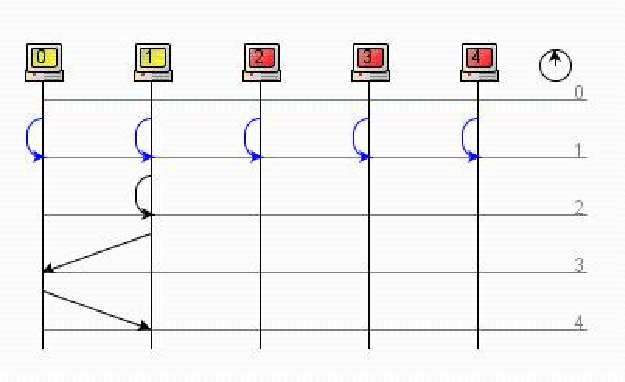
\includegraphics{images/p1ReadSeq.pdf}
	\caption{Bezeichnung der Abbildung}
	\label{a1}
\end{figure}

\begin{table} %[hbtp]
	\centering
		\begin{tabular}{l | l l l l}
		\textbf{Prozesse} & \textbf{Zeit} $\rightarrow$ \\
		\hline
			$P_{1}$ & $W(x)1$ \\
			$P_{2}$ & & $W(x)2$ \\
			$P_{3}$ & & $R(x)2$ & & $R(x)1$\\
			$P_{4}$ & & & $R(x)2$ & $R(x)1$\\
		\end{tabular}
	\caption{Bezeichnung der Tabelle}
	\label{t1}
\end{table}


\section{Mathematische Formel}\index{Formel}
Mathematische Formeln bzw. Formulierungen k�nnen sowohl im
laufenden Text (z.B. $y=x^2$) oder abgesetzt und zentriert im Text
erscheinen. Gleichungen sollten f�r Referenzierungen nummeriert
werden (siehe Formel \ref{gl-1}).
\begin{equation}
\label{gl-1}
e_{i}=\sum _{i=1}^{n}w_{i}x_{i}
\end{equation}

Entscheidungsformel:

\begin{equation}
\psi(t)=\left\{\begin{array}{ccc}
1 &  \qquad 0 <= t < \frac{1}{2} \\
-1 &  \qquad \frac{1}{2} <= t <1 \\
0 & \qquad sonst
\end{array} \right.
\end{equation}


Matrix:\index{Matrix}
\begin{equation}
A = \left(
\begin{array}{llll}
a_{11} & a_{12} & \ldots & a_{1n} \\
a_{21} & a_{22} & \ldots & a_{2n} \\
\vdots & \vdots & \ddots & \vdots \\
a_{n1} & a_{n2} & \ldots & a_{nn} \\
\end{array}
\right)
\end{equation}

Vektor:\index{Vektor} 

\begin{equation}
\overline{a} = \left(
\begin{array}{c}
a_{1}\\
a_{2}\\
\vdots\\
a_{n}\\
\end{array}
\right)
\end{equation}

\section{S�tze, Lemmas und Definitionen}\index{Satz}\index{Lemma}\index{Definition}

S�tze, Lemmas, Definitionen, Beweise,\index{Beweis} Beispiele\index{Beispiel} k�nnen in speziell daf�r vorgesehenen Umgebungen erstellt werden.

\begin{definition}(Optimierungsproblem)

Ein \emph{Optimierungsproblem} $\mathcal{P}$ ist festgelegt durch ein Tupel
$(I_\mathcal{P}, sol_\mathcal{P}, m_\mathcal{P}, goal)$ wobei gilt

\begin{enumerate}
\item $I_\mathcal{P}$ ist die Menge der Instanzen,
\item $sol_\mathcal{P} : I_\mathcal{P} \longmapsto \mathbb{P}(S_\mathcal{P})$ ist eine Funktion, die jeder Instanz $x \in I_\mathcal{P}$ eine Menge zul�ssiger L�sungen zuweist,
\item $m_\mathcal{P} : I_\mathcal{P} \times S_\mathcal{P} \longmapsto \mathbb{N}$ ist eine Funktion, die jedem Paar $(x,y(x))$ mit $x \in I_\mathcal{P}$ und $y(x) \in sol_\mathcal{P}(x)$ eine
Zahl $m_\mathcal{P}(x,y(x)) \in \mathbb{N}$ zuordnet (= Ma� f�r die L�sung $y(x)$ der Instanz $x$), und
\item $goal \in \{min,max\}$.
\end{enumerate}

\end{definition}

\begin{example} MINIMUM TRAVELING SALESMAN (MIN-TSP)
\begin{itemize}
\item $I_{MIN-TSP} =_{def}$ s.o., ebenso $S_{MIN-TSP}$
\item $sol_{MIN-TSP}(m,D) =_{def} S_{MIN-TSP} \cap \mathbb{N}^m$ 
\item $m_{MIN-TSP}((m,D),(c_1, \ldots , c_m)) =_{def} \sum_{i=1}^{m-1} D(c_i, c_{i+1}) + D(c_m,c_1)$ 
\item $goal_{MIN-TSP} =_{def} min$
\end{itemize}
\begin{flushright}
$\qed$
\end{flushright}
\end{example}

\begin{theorem} Sei $\mathcal{P}$ ein \textbf{NP}-hartes Optimierungsproblem.
Wenn $\mathcal{P} \in$ \textbf{PO}, dann ist \textbf{P} = \textbf{NP}.
\end{theorem}

\begin{proof} Um zu zeigen, dass \textbf{P} = \textbf{NP} gilt, gen�gt es
wegen Satz A.30 zu zeigen, dass ein einziges \textbf{NP}-vollst�ndiges
Problem in \textbf{P} liegt. Sei also $\mathcal{P}'$ ein beliebiges \textbf{NP}-vollst�ndiges Problem.

Weil $\mathcal{P}$ nach Voraussetzung \textbf{NP}-hart ist, gilt insbesondere
$\mathcal{P}' \leq_T \mathcal{P}_C$. Sei $R$ der zugeh�rige
Polynomialzeit-Algorithmus dieser Turing-Reduktion.
Weiter ist $\mathcal{P} \in$ \textbf{PO} vorausgesetzt, etwa verm�ge eines
Polynomialzeit-Algorithmus $A$. Aus den beiden
Polynomialzeit-Algorithmen $R$ und $A$ erh�lt man nun
leicht einen effizienten Algorithmus f�r $\mathcal{P}'$: Ersetzt man
in $R$ das Orakel durch $A$, ergibt dies insgesamt eine polynomielle
Laufzeit. 
%\begin{flushright}
$\qed$
% \end{flushright}
\end{proof}

\begin{lemma} Aus \textbf{PO} $=$ \textbf{NPO} folgt \textbf{P} $=$ \textbf{NP}.
\end{lemma}

\begin{proof} Es gen�gt zu zeigen, dass unter der angegeben
Voraussetzung KNAPSACK $\in$ \textbf{P} ist.

Nach Voraussetung ist MAXIMUM KNAPSACK $\in$ \textbf{PO},
d.h. die Berechnung von $m^*(x)$ f�r jede Instanz $x$ ist
in Polynomialzeit m�glich. Um KNAPSACK bei Eingabe
$(x,k)$ zu entscheiden, m�ssen wir nur noch $m^*(x) \geq k$
pr�fen. Ist das der Fall, geben wir $1$, sonst $0$ aus. Dies
bleibt insgesamt ein Polynomialzeit-Algorithmus. 
\begin{flushright}
$\qed$
\end{flushright}
\end{proof}

\section{Fu�noten}

In einer Fu�note k�nnen erg�nzende Informationen\footnote{Informationen die f�r die Arbeit zweitrangig sind, jedoch f�r den Leser interessant sein k�nnten.} angegeben werden. Au�erdem kann eine Fu�note auch Links enthalten. Wird in der Arbeit eine Software (zum Beispiel Java-API\footnote{\url{http://java.sun.com/}}) eingesetzt, so kann die Quelle, die diese Software zur Verf�gung stellt in der Fu�note angegeben werden.

\section{Literaturverweise}\index{Literatur}
Alle benutzte Literatur wird im Literaturverzeichnis angegeben\footnote{Dazu wird ein sogennanter bib-File, literatur.bib verwendet.}. Alle angegebene Literatur sollte mindestens einmal im Text referenziert werden\cite{Coulouris:02}.
\chapter{Beispiel-Kapitel}

In diesem Kapitel wird beschrieben, warum es unterschiedliche Konsistenzmodelle\index{Konsistenzmodelle} gibt. Au�erdem werden die Unterschiede zwischen strengen Konsistenzmodellen\index{Linearisierbarkeit} (Linearisierbarkeit, sequentielle Konsistenz)\index{sequentiell!Konsistenz} und schwachen Konsistenzmodellen\index{Konsistenz!schwach} (schwache Konsistenz, Freigabekonsistenz)\index{Freigabekonsistenz} erl�utert. Es wird gekl�rt, was Strenge und Kosten (billig, teuer) in Zusammenhang mit Konsistenzmodellen bedeuten.

\section{Warum existieren unterschiedliche Konsistenzmodelle?}

Laut \cite{Malte:97} sind mit der\index{Replikation} Replikation von Daten immer zwei gegens�tzliche Ziele verbunden: die Erh�hung der\index{Verf�gbarkeit} Verf�gbarkeit und die Sicherung der\index{Konsistenz} Konsistenz der Daten. Die Form der Konsistenzsicherung bestimmt dabei, inwiefern das eine Kriterium erf�llt und das andere dementsprechend nicht erf�llt ist (Trade-off zwischen Verf�gbarkeit und der Konsistenz der Daten). Stark konsistente Daten sind stabil, das hei�t, falls mehrere Kopien der Daten existieren, d�rfen keine Abweichungen auftreten. Die Verf�gbarkeit der Daten ist hier jedoch stark eingeschr�nkt. Je schw�cher die Konsistenz wird, desto mehr Abweichungen k�nnen zwischen verschiedenen Kopien einer Datei auftreten, wobei die Konsistenz nur an bestimmten Synchronisationspunkten gew�hrleistet wird. Daf�r steigt aber die Verf�gbarkeit der Daten, weil sie sich leichter replizieren lassen.

Nach \cite{Mosberger:93} kann die Performanzsteigerung der schw�cheren Konsistenzmodelle wegen der Optimierung\index{Optimierung} (Pufferung, Code-Scheduling, Pipelines) 10-40 Prozent betragen. Wenn man bedenkt, dass mit der Nutzung der vorhandenen Synchronisierungsmechanismen schw�chere Konsistenzmodelle den Anforderungen der strengen Konsistenz gen�gen, stellt sich der h�here programmiertechnischer Aufwand bei der Implementierung der schw�cheren Konsistenzmodelle als ihr einziges Manko dar.

In \cite{Cheriton:85} ist beschrieben, wie man sich Formen von DSM vorstellen k�nnte, f�r die ein beachtliches Ma� an\index{Inkonsistenz} Inkonsistenz akzeptabel w�re. Beispielsweise k�nnte DSM verwendet werden, um die Auslastung von Computern in einem Netzwerk zu speichern, so dass Clients f�r die Ausf�hrung ihrer Applikationen die am wenigsten ausgelasteten Computer ausw�hlen k�nnen. Weil die Informationen dieser Art innerhalb k�rzester Zeit ungenau werden k�nnen (und durch die Verwendung der veralteten Daten keine gro�en Nachteile entstehen k�nnen), w�re es vergebliche M�he, sie st�ndig f�r alle Computer im System konsistent zu halten \cite{Coulouris:02}. Die meisten Applikationen stellen jedoch strengere Konsistenzanforderungen.

\section{Klassifizierung eines Konsistenzmodells}

Die zentrale Frage, die f�r die Klassifizierung\index{streng}\index{schwach} (streng oder schwach) eines Konsistenzmodells von Bedeutung ist \cite{Coulouris:02}: wenn ein Lesezugriff auf eine Speicherposition erfolgt, welche Werte von Schreibzugriffen auf diese Position sollen dann dem Lesevorgang bereitgestellt werden? Die Antwort f�r das schw�chste Konsistenzmodell lautet: von jedem Schreibvorgang, der vor dem Lesen erfolgt ist, oder in der "`nahen"' Zukunft, innerhalb des definierten Betrachtungsraums, erfolgten wird. Also irgendein Wert, der vor oder nach dem Lesen geschrieben wurde.

F�r das strengste Konsistenzmodell, Linearisierbarkeit (atomic consistency), stehen alle geschriebenen Werte allen Prozessoren sofort zur Verf�gung: eine Lese-Operation gibt den aktuellsten Wert zur�ck, der geschrieben wurde, bevor das Lesen stattfand. Diese Definition ist aber in zweierlei Hinsicht problematisch. Erstens treten weder Schreib- noch Lese-Operationen zu genau einem Zeitpunkt auf, deshalb ist die Bedeutung von "`aktuellsten"' nicht immer klar. Zweitens ist es nicht immer m�glich, genau festzustellen, ob ein Ereignis vor einem anderen stattgefunden hat, da es Begrenzungen daf�r gibt, wie genau Uhren in einem verteilten System synchronisiert werden k�nnen.

Nachfolgend werden einige Konsistenzmodelle absteigend nach ihrer Strenge vorgestellt. Zuvor m�ssen wir allerdings kl�ren, wie die Lese- und Schreibe-Operationen in dieser Ausarbeitung dargestellt werden.

Sei $x$ eine Speicherposition, dann k�nnen Instanzen dieser Operationen wie folgt ausgedr�ckt werden:
\begin{itemize}
	\item $R(x)a$ - eine Lese-Operation\index{Operation!Lese}, die den Wert $a$ von der Position $x$ liest.
	\item $W(x)b$ - eine Schreib-Operation\index{Operation!Schreib}, die den Wert $b$ an der Position $x$ speichert.
\end{itemize}

\section{Linearisierbarkeit\index{Linearisierbarkeit} (atomic consistency)}

Die Linearisierbarkeit im Zusammenhang mit DSM kann wie folgt definiert werden:
\begin{itemize}
	\item Die verzahnte Operationsabfolge findet so statt: wenn $R(x)a$ in der Folge vorkommt, dann ist die letzte Schreib-Operation, die vor ihr in der verzahnten Abfolge auftritt, $W(x)a$, oder es tritt keine Schreib-Operation vor ihr auf und $a$ ist der Anfangswert von $x$. Das bedeutet, dass eine Variable nur durch eine Schreib-Operation ge�ndert werden kann.
	\item Die Reihenfolge der Operationen in der Verzahnung ist konsistent zu den \underline{Echtzeiten}\index{Echtzeiten}, zu denen die Operationen bei der tats�chlichen Ausf�hrung aufgetreten sind.
\end{itemize}

Die Bedeutung dieser Definition kann an folgendem Beispiel (Tabelle \ref{tab:1}) nachvollzogen werden. Es sei angenommen, dass alle Werte mit $0$ vorinitialisiert sind.

\begin{table}
	\centering
		\begin{tabular}{l | l l l l}
			\textbf{Prozesse} & \textbf{Zeit} $\rightarrow$ & \\
			\hline
			$P_{1}$ & $W(x)1$ & & $W(y)2$ \\
			$P_{2}$ & & $R(x)1$ & & $R(y)2$ \\
		\end{tabular}
	\caption{Linearisierbarkeit ist erf�llt}
	\label{tab:1}
\end{table}

Hier sind beide Bedingungen erf�llt, da die Lese-Operationen den zuletzt geschriebenen Wert zur�ckliefern. Interessanter ist es, zu sehen, wann die Linearisierbarkeit verletzt ist.

\begin{table}
	\centering
		\begin{tabular}{l | l l l l}
		\textbf{Prozesse} & \textbf{Zeit} $\rightarrow$ \\
		\hline
		$P_{1}$ & $W(x)1$ & $W(x)2$ \\
		$P_{2}$ & & & \color{red} $R(x)0$ & \color{black} $R(x)2$ \\
		\end{tabular}
	\caption{Linearisierbarkeit ist verletzt, sequentielle Konsistenz ist erf�llt.}
	\label{tab:2}
\end{table}

In diesem Beispiel (Tabelle \ref{tab:2}) ist die Echtzeit-Anforderung verletzt, da der Prozess $P_{2}$ immer noch den alten Wert liest, obwohl er von Prozess $P_{1}$ bereits ge�ndert wurde. Diese Ausf�hrung w�re aber sequentiell konsistent (siehe kommender Abschnitt), da es eine Verzahnung der Operationen gibt, die diese Werte liefern k�nnte ($R(x)0$, $W(x)1$, $W(x)2$, $R(y)2$). W�rde man beide Lese-Operationen des 2. Prozesses vertauschen, wie in der Tabelle \ref{tab:3} dargestellt, so w�re keine sinnvolle Verzahnung mehr m�glich.

\begin{table}
	\centering
		\begin{tabular}{l | l l l l}
		\textbf{Prozesse} & \textbf{Zeit} $\rightarrow$ \\
		\hline
		$P_{1}$ & $W(x)1$ & $W(x)2$ \\
		$P_{2}$ & & & \color{red} $R(x)2$ &  \color{red} $R(x)0$ \\
			
		\end{tabular}
	\caption{Linearisierbarkeit und sequentielle Konsistenz sind verletzt.}
	\label{tab:3}
\end{table}

In diesem Beispiel sind beide Bedingungen verletzt. Selbst wenn die Echtzeit, zu der die Operationen stattgefunden haben, ignoriert wird, gibt es keine Verzahnung einzelner Operationen, die der Definition entsprechen w�rde.
\chapter{Zusammenfassung und Ausblick}

%In diesem Kapitel soll die Arbeit noch einmal kurz zusammengefasst werden. Insbesondere sollen die wesentlichen Ergebnisse Ihrer Arbeit herausgehoben werden. Erfahrungen, die z.B. Benutzer mit der Mensch-Maschine-Schnittstelle gemacht haben oder Ergebnisse von Leistungsmessungen sollen an dieser Stelle pr�sentiert werden. Sie k�nnen in diesem Kapitel auch die Ergebnisse oder das Arbeitsumfeld Ihrer Arbeit kritisch bewerten. W�nschenswerte Erweiterungen sollen als Hinweise auf weiterf�hrende Arbeiten erw�hnt werden.


\section{Zusammenfassung}

Im Kapitel Einleitung und Problemstellung wurde die Aufgabenstellung erl�utert, wobei sich bereits zeigte dass diese aufgrund des semistrukturierten Aufbaus der zu durchsuchenden Dokumente eine sehr spezifische L�sung erfordern w�rde. Die Unterteilung in Metadaten und Freitext sowie das logische Verkn�pfen der Suchbedingungen stellen die wesentlichen Herausforderungen dar.
Anschlie�end wurden die notwendigen theoretischen Kenntnisse vermittelt. Die Bedeutung des Begriffs Information Retrieval wurde erkl�rt und es zeigte sich, dass diese sehr weit gefasst ist,  weshalb diese Arbeit die ausgesprochen umfangreiche Thematik nur ansatzweise behandeln kann. Es wurden die beiden bekanntesten klassichen Information Retrieval  Verfahren vorgestellt; das boolesche Retrieval und das Vektorraummodell, sowie Methoden, anhand derer sich solche Modelle im Hinblick auf Qualit�t bewerten und Vergleichen lassen. Hierbei zeigte sich, dass eine solche Bewertung im Rahmen dieser Arbeit aufgrund des Aufwands leider nicht durchf�hrbar ist. \\
Im Implementierungskapitel wurde deutlich, dass die Verwendung eines der beiden klassischen Verfahren nicht ausreicht, die Kombination aus booleschen Retrieval und Vektorraummodell jedoch hervorragend passt. Das boolesche Retrieval musste allerdings geringf�gig modifiziert werden, indem nicht nur das Vorkommen der Attribute in den Dokumenten vermerkt wird, sondern auch deren Inhalt inklusive Datentyp. Beim Vektorraummodell zeigte sich, dass sich Speicher sparen l�sst, indem alle Elemente des Vektors, welche eine 0 enthalten, nicht eingetragen werden. \\
Zuletzt zeigte sich, dass die Benutzeroberfl�che eine nicht zu untersch�tzende Herausforderung darstellt,
da der Anwender sein Informationsbed�rfnis auf m�glichst unkomplizierte Art ausdr�cken k�nnen soll. Ein Information Retrieval System muss vom Nutzer auch verstanden werden. Es wurde sich daf�r entschieden, m�glichst einfache UI-Elemente wie CheckBoxes zu w�hlen sowie die Oberfl�che in drei thematische Bereiche zu gliedern, um die notwendige �bersicht zu bieten.




 \section{Ausblick: W�nschenswerte Erweiterungen}
Einige Erweiterungen konnten aus zeitlichen Gr�nden in der Implementierung nicht umgesetzt werden, sind jedoch w�nschenswert. \\
Die Im Kapitel Grundbegriffe beschriebene Lemmatisierung (siehe Abschnitt \ref{lemmatisierung}) w�rde eine gro�e Verbesserung hinsichtlich des Speicherbedarfs bedeuten, da weniger Terme gespeichert werden m�ssen. Zudem w�rde das Erg�nzen um Lemmatisierung auch die Suche verbessern, da auch Dokumente mit zum Suchbegriff verwandten W�rtern als Treffer gewertet werden. \\
Weiterhin w�nschenswert ist die Erg�nzung um Spelling Correction, d.h. um eine Rechtschreibkorrektur die �hnliche Suchbegriffe vorschl�gt, falls der Anwender sich bei der Eingabe vertippt hat. Dies w�rde die Anwenderfreundlichkeit des Systems erheblich steigern, insbesondere in F�llen in welchen der Anwender seinen Tippfehler nicht bemerkt und unerwartet keine Resultate erh�lt. Da Nutzer in der Regel Spelling Correction aus der allt�glichen Websuche gew�hnt sind, ist es w�nschenswert auch dieses Information Retrieval System damit auszustatten.


%-Stopwords \\
%-Lemmatisierung \\
%-Spelling Correction \\

% ...
%--------------------------------------------------------------------------
\backmatter                        		% Anhang
%-------------------------------------------------------------------------
\bibliographystyle{geralpha}			% Literaturverzeichnis
\bibliography{literatur}     			% BibTeX-File literatur.bib
%--------------------------------------------------------------------------
\printindex 							% Index (optional)
%--------------------------------------------------------------------------
\begin{appendix}						% Anh�nge sind i.d.R. optional
   \chapter{Glossar}

\abbreviation{DisASTer}		{DisASTer (Distributed Algorithms Simulation Terrain), A platform for the Implementation of Distributed Algorithms}
\abbreviation{DSM}			{Distributed Shared Memory}
\abbreviation{AC}			{Linearisierbarkeit (atomic consistency)}
\abbreviation{SC}			{Sequentielle Konsistenz (sequential consistency)}
\abbreviation{WC}			{Schwache Konsistenz (weak consistency)}
\abbreviation{RC}			{Freigabekonsistenz (release consistency)}
			% Glossar   
   \chapter{Erkl�rung der Kandidatin / des Kandidaten}

\begin{description}[$\Box$~]
\item[$\Box$] Die Arbeit habe ich selbstst�ndig verfasst und keine anderen als die angegebenen Quellen- und Hilfsmittel verwendet.\\

\item[$\Box$] Die Arbeit wurde als Gruppenarbeit angefertigt. Meine eigene Leistung ist\\
...\\

Diesen Teil habe ich selbstst�ndig verfasst und keine anderen als die angegebenen Quellen und Hilfsmittel verwendet. \\

Namen der Mitverfasser: ...

\end{description}

\vspace{2cm}

\begin{minipage}[t]{3cm}
\rule{3cm}{0.5pt}
Datum
\end{minipage}
\hfill
\begin{minipage}[t]{9cm}
\rule{9cm}{0.5pt}
Unterschrift der Kandidatin / des Kandidaten
\end{minipage}	% Selbstst�ndigkeitserkl�rung
\end{appendix}

\end{document}
